% Hlavicka pro protokoly z fyzikalniho praktika.
% Verze pro: LaTeX
% Verze hlavicky: 22. 2. 2007
% Autor: Ustav fyziky kondenzovanych latek
% Ke stazeni: www.physics.muni.cz/ufkl/Vyuka/
% Licence: volne k pouziti, nejlepe k vcasnemu odevzdani protokolu z Vaseho mereni.


\documentclass[czech,11pt,a4paper]{article}
\usepackage[T1]{fontenc}
\usepackage{graphicx}
\usepackage{mathtools}
\usepackage{amssymb}
\usepackage{amsthm}
\usepackage{thmtools}
\usepackage{xcolor}
\usepackage{nameref}
\usepackage{babel}
\usepackage{hyperref}
\usepackage{multicol}
\usepackage[export]{adjustbox}
\usepackage{subcaption}
\usepackage{caption}
\usepackage{multirow}
\usepackage{float}
\usepackage{placeins}




%%% Nemente:
\usepackage[margin=2cm]{geometry}
\newtoks\jmenopraktika \newtoks\jmeno \newtoks\datum
\newtoks\obor \newtoks\skupina \newtoks\rocnik \newtoks\semestr
\newtoks\cisloulohy \newtoks\jmenoulohy
\newtoks\tlak \newtoks\teplota \newtoks\vlhkost
%%% Nemente - konec.


%%%%%%%%%%% Doplnte pozadovane polozky:

\jmenopraktika={Fyzikální praktikum 2}  % nahradte jmenem vaseho predmetu
\jmeno={Teodor Duraković}            % nahradte jmenem mericiho
\datum={7.~října 2024}        % nahradte datem mereni ulohy
\obor={F}                     % nahradte zkratkou vami studovaneho oboru
\skupina={Po 14:00}            % nahradte dobou vyuky vasi seminarni skupiny
\rocnik={II}                  % nahradte rocnikem, ve kterem studujete
\semestr={III}                 % nahradte semestrem, ve kterem studujete

\cisloulohy={2}               % nahradte cislem merene ulohy
\jmenoulohy={Tranzistor a zesilovač napětí} % nahradte jmenem merene ulohy

\tlak={985}                   % nahradte tlakem pri mereni (v hPa)
\teplota={23.0}               % nahradte teplotou pri mereni (ve stupnich Celsia)
\vlhkost={43}               % nahradte vlhkosti vzduchu pri mereni (v %)

%%%%%%%%%%% Konec pozadovanych polozek.


%%%%%%%%%%% Uzitecne balicky:

%%%%%% Zamezeni parchantu:
\widowpenalty 10000 \clubpenalty 10000 \displaywidowpenalty 10000
%%%%%% Parametry pro moznost vsazeni vetsiho poctu obrazku na stranku
\setcounter{topnumber}{3}	  % max. pocet floatu nahore (specifikace t)
\setcounter{bottomnumber}{3}	  % max. pocet floatu dole (specifikace b)
\setcounter{totalnumber}{6}	  % max. pocet floatu na strance celkem
\renewcommand\topfraction{0.9}	  % max podil stranky pro floaty nahore
\renewcommand\bottomfraction{0.9} % max podil stranky pro floaty dole
\renewcommand\textfraction{0.1}	  % min podil stranky, ktery musi obsahovat text
\intextsep=8mm \textfloatsep=8mm  %\intextsep pro ulozeni [h] floatu a \textfloatsep pro [b] or [t]

% Tecky za cisly sekci:
\renewcommand{\thesection}{\arabic{section}.}
\renewcommand{\thesubsection}{\thesection\arabic{subsection}.}
\renewcommand{\thesubsubsection}{\thesubsection\arabic{subsubsection}.}
% Jednopismenna mezera mezi cislem a nazvem kapitoly:
\makeatletter \def\@seccntformat#1{\csname the#1\endcsname\hspace{1ex}} \makeatother


%%%%%%%%%%%%%%%%%%%%%%%%%%%%%%%%%%%%%%%%%%%%%%%%%%%%%%%%%%%%%%%%%%%%%%%%%%%%%%%
%%%%%%%%%%%%%%%%%%%%%%%%%%%%%%%%%%%%%%%%%%%%%%%%%%%%%%%%%%%%%%%%%%%%%%%%%%%%%%%
% Zacatek dokumentu
%%%%%%%%%%%%%%%%%%%%%%%%%%%%%%%%%%%%%%%%%%%%%%%%%%%%%%%%%%%%%%%%%%%%%%%%%%%%%%%
%%%%%%%%%%%%%%%%%%%%%%%%%%%%%%%%%%%%%%%%%%%%%%%%%%%%%%%%%%%%%%%%%%%%%%%%%%%%%%%

\begin{document}
	
	%%%%%%%%%%%%%%%%%%%%%%%%%%%%%%%%%%%%%%%%%%%%%%%%%%%%%%%%%%%%%%%%%%%%%%%%%%%%%%%
	% Nemente:
	%%%%%%%%%%%%%%%%%%%%%%%%%%%%%%%%%%%%%%%%%%%%%%%%%%%%%%%%%%%%%%%%%%%%%%%%%%%%%%%
	\thispagestyle{empty}
	
	{
		\begin{center}
			\sf 
			{\Large Ústav fyzikální elektroniky Přírodovědecké fakulty Masarykovy univerzity} \\
			\bigskip
			{\huge \bfseries FYZIKÁLNÍ PRAKTIKUM} \\
			\bigskip
			{\Large \the\jmenopraktika}
		\end{center}
		
		\bigskip
		
		\sf
		\noindent
		\setlength{\arrayrulewidth}{1pt}
		\begin{tabular*}{\textwidth}{@{\extracolsep{\fill}} l l}
			\large {\bfseries Zpracoval:}  \the\jmeno & \large  {\bfseries Naměřeno:} \the\datum\\[2mm]
			\large  {\bfseries Obor:} \the\obor  \hspace{40mm}  {\bfseries Skupina:} \the\skupina %
			%{\bfseries Ročník:} \the\rocnik \hspace{5mm} {\bfseries Semestr:} \the\semestr  
			&\large {\bfseries Testováno:}\\
			\\
			\hline
		\end{tabular*}
	}
	
	\bigskip
	
	{
		\sf
		\noindent \begin{tabular}{p{3cm} p{0.6\textwidth}}
			\Large  Úloha č. {\bfseries \the\cisloulohy:} \par
			\smallskip
			$T=\the\teplota$~$^\circ$C \par
			$p=\the\tlak$~hPa \par
			$\varphi=\the\vlhkost$~\%
			&\Large \bfseries \the\jmenoulohy  \\[2mm]
		\end{tabular}
	}
	
	\vskip1cm
	
	%%%%%%%%%%%%%%%%%%%%%%%%%%%%%%%%%%%%%%%%%%%%%%%%%%%%%%%%%%%%%%%%%%%%%%%%%%%%%%%
	% konec Nemente.
	%%%%%%%%%%%%%%%%%%%%%%%%%%%%%%%%%%%%%%%%%%%%%%%%%%%%%%%%%%%%%%%%%%%%%%%%%%%%%%%
	
	%%%%%%%%%%%%%%%%%%%%%%%%%%%%%%%%%%%%%%%%%%%%%%%%%%%%%%%%%%%%%%%%%%%%%%%%%%%%%%%
	%%%%%%%%%%%%%%%%%%%%%%%%%%%%%%%%%%%%%%%%%%%%%%%%%%%%%%%%%%%%%%%%%%%%%%%%%%%%%%%
	% Zacatek textu vlastniho protokolu
	%%%%%%%%%%%%%%%%%%%%%%%%%%%%%%%%%%%%%%%%%%%%%%%%%%%%%%%%%%%%%%%%%%%%%%%%%%%%%%%
	%%%%%%%%%%%%%%%%%%%%%%%%%%%%%%%%%%%%%%%%%%%%%%%%%%%%%%%%%%%%%%%%%%%%%%%%%%%%%%%
	
	\begin{multicols}{2}
	\section{Zadání}
	1. Změřit převodní a výstupní charakteristiku tranzistoru.\\
	2. Z charakteristik určit parametry tranzistoru $S, R_i, \mu $ ve zvoleném pracovním bodě.\\
	3. Zvolit napájecí napětí $E$ a zatěžovací odpor $R_Z$.\\
	4. Pozorovat vliv amplitudy střídavého napětí generátoru na tvar výstupního napětí.\\
	6. Vypočítat zesílení $A_V$ a $A_G$.\\
	\section{Úvod}
	Unipolární tranzistor je prvek nelineární, jeho odpor se tudíž neřídí Ohmovým zákonem a jeho voltampérová charakteristika je nelineární. Voltampérovou charakteristiku lze u tohoto typu tranzistoru ovlivňovat napětím hradla (gatu). Tento prvek lze popsat třemi obecně nelineárními charakteristikami: Vstupní, výstupní a převodní charakteristikou.\\V této úloze vybereme unipolární tranzistor, u kterého změříme převodní a výstupní charakteristiky a z nich pak určíme parametry tranzistoru. Dále pak sestavíme z tranzistoru napětový zesilovač a změříme jeho napětové zesílení. To pak porovnáme se zesílením vypočteným z naměřených charakteristik.
	\section{Postup, metody měření}
	Proud $I_D$ protékající ze zdroje v obvodu mezi drain (D) a source (S) lze regulovat napětím na hradle (gatu )$U_G$. 
	Při použití tranzistoru jako zesilovače se při provozu pohybujeme v okolí určitého pracovního bodu (hodnoty napětí na hradle $U_{G}$ a drain $U_{D}$ se mění jen v omezeném rozsahu). Nelineární charakteristiku pak můžeme aproximativně linearizovat. Zavádíme tak veličiny strmost, vnitřní odpor a zesilovací činitel, které však závisí na zvoleném pracovním bodě. Pracovní bod $P$ definejme pomocí dvojice hodnot: napětí na hradle $U_{G 0}$ na drainu $U_{D 0}$. Proud v tomto pracovním bodě označíme $I_{D 0}$.
	Derivace převodní charakteristiky podle hradlového napětí $U_{G}$ se nazývá statická strmost tranzistoru $S$
	
	\begin{equation}
		S=\left.\frac{\partial I_{D}}{\partial U_{G}}\right|_{U_{D}=\text { konst. }} 
	\end{equation}
	
	
	Nejlépe ji určíme jako směrnici přímky proložené několika body v okolí pracovního bodu $P$. Použijeme alespoň dva body na každou stranu od pracovního bodu, tedy celkem alespoň pět bodů. Použijeme-li více bodů bude výsledek méně ovlivněn šumem v experimentálních datech, prokládaný interval je však třeba zvolit tak, aby se v něm naměřená charakteristika příliš neodchylovala od lineární závislosti. Převrácená hodnota derivace výstupní charakteristiky podle napětí na drainu je rovna vnitřnímu odporu tranzistoru $R_{i}$ :
	
	\begin{equation}
		R_{i}=\left.\frac{\partial U_{D}}{\partial I_{D}}\right|_{U_{G}=\text { konst. }} 
	\end{equation}
	
	který určíme obdobným způsobem jako strmost, tedy proložením přímky výstupní charakteristikou v okolí pracovního bodu $P$. Dalšími užívanými charakteristikami tranzistoru v pracovním bodě jsou zesilovací činitel tranzistoru $\mu$ :
	
	\begin{equation}
		\mu=\left.\frac{\partial U_{D}}{\partial U_{G}}\right|_{I_{D}=\text { konst. }}
	\end{equation}
	Takto definované veličiny splňují Barkhausenovu rovnici
	\begin{equation}
		SR_i\frac 1 \mu = 1.
	\end{equation}
	Známe-li dva z těchto parametru, třetí můžeme z rovnice vypočítat. To použijeme pro kalkulaci hodnoty zesilovacího činitele, jelikož měření charakteristiky s konstantním proudem je experimentálně obtížné a tato data nemáme k disposici.
	K měření uvedených závislostí tranzistor zapojíme dle obrázku 1:
	\begin{figure}[H]
		\begin{center}
			
			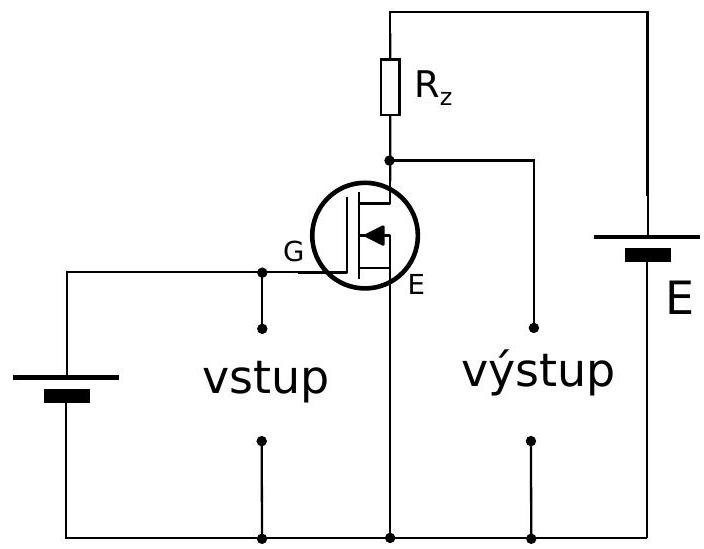
\includegraphics[width=0.8\linewidth, ]{zapojeni1} 
			\caption{Zapojení tranzistoru}
		\end{center}
		
	\end{figure} 
	\subsection{Tranzistor jako zesilovač napětí}
	Při zapojení tranzistoru jako zesilovače napětí je důležitý i zatěžovací/pracovní odpor $R_z$. Na zapojení uvedené na obr. 1 můžeme hledět jako na napěťový dělič, kdy napětí na tranzistoru $U_D$ a odporu $R_zI_D$ v součtu dávají napětí zdroje $E$. Zvýšením napětí na hradle vzroste proud tranzistorem, což můžeme interpretovat jako pokles jeho odporu. 
	Platí formule
	\begin{equation}
		E-I_DR_z-U_D = 0,
	\end{equation}
	kterou můžeme upravit na
	\begin{equation}
		R_Z = \frac{E-U_{D0}}{I_{D0}}
	\end{equation}
	Tuto formuli použijeme pro nastavení zesilovače do zadaného pracovního bodu, kde je potřeba zvolit $E$, resp. $R_z$. Platí, že největšího napěťového zesílení dosáhneme, pokud bude napětí zdroje $E$ rovno zhruba dvojnásobku hodnoty $U_D0$
	Protože máme k dispozici změřenou sadu výstupních charakteristik tranzistoru, můžeme zesílení určit také graficky. Nejprve rovnici 2.12 přepíšeme do tvaru tzv. zatěžovací přímky
	
	\begin{equation}
		I_{D}=\frac{E-U_{D}}{R_{z}}
	\end{equation}
	
	která vyjadřuje závislost proudu protékajícího rezistorem na výstupním napětí $U_{D}$. Tento proud musí být shodný s proudem $I_{D}$ tekoucím tranzistorem vyjádřeným funkcí (2.9). Zakreslíme-li zatěžovací přímku do grafu výstupních charakteristik, budou průsečíky zatěžovací přímky s výstupními charakteristikami parametrizovanými hradlovým napětím $U_{G}$ určovat závislost napětí na výstupu zesilovače $U_{D}$ na vstupním napětí $U_{D}$ v okolí pracovního bodu $P, \mathrm{tj} . U_{D 0}, I_{D 0}$. Pomocí této konstrukce můžeme také určit zesílení tranzistorového zesilovače.
	
	\begin{equation}
		A_{G}=\frac{\Delta U_{D}}{\Delta U_{G}} 
	\end{equation}
  	Při zesílení signálu z generátoru střídavého napětí získáme hodnotu zesílení jako podíl amplitud výstupního a vstupního napětí:
  	\begin{equation}
  		A_M = \frac{u_{m2}}{u_{m1}}
  	\end{equation}
  	Zesílení tranzistoru $A_V$ získáme formulí:
  	
  	\begin{equation}
  		A_V = \frac{SR_z}{1+ \frac{R_i}{R_z}}
  	\end{equation}
  	
	\section{Měření}
		\begin{figure}[H]
		\begin{center}
			
			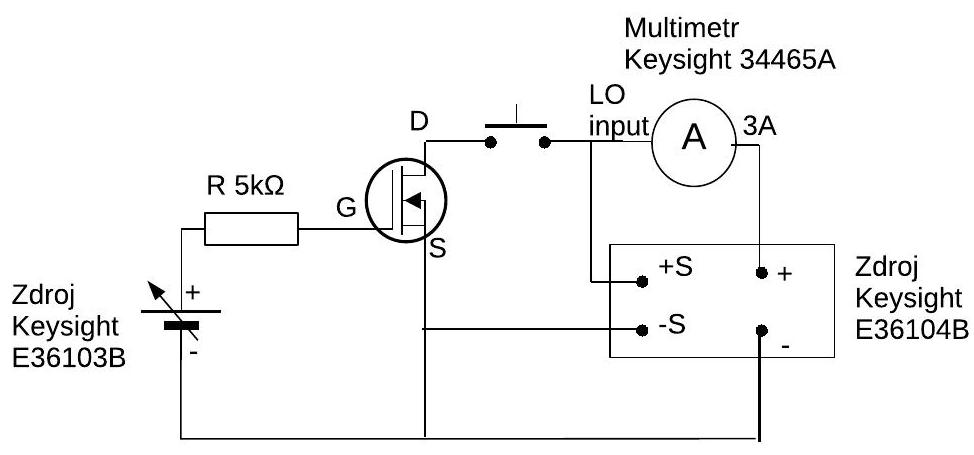
\includegraphics[width=1\linewidth, ]{zapojeni2} 
			\caption{Zapojení pro měření statických charakteristik.}
		\end{center}		
	\end{figure} 
	Dle Obr. 2. zapojíme měřicí přístroje a ostatní komponenty. Ručně změříme jednu převodní charakteristiku při $U_D=const.=10V$ a jednu výstupní charakteristiku při $U_G=const.=3.6V$. Získáváme:
	\begin{figure}[H]
		\begin{center}			
			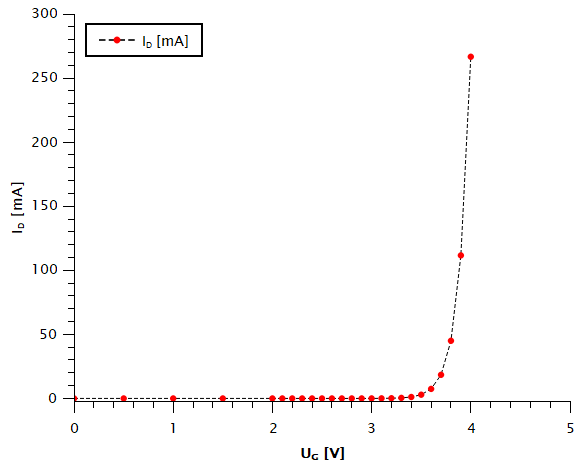
\includegraphics[width=0.8\linewidth, ]{prevod1} 
			\caption{Převodní charakteristika při $U_D = 10V$}
			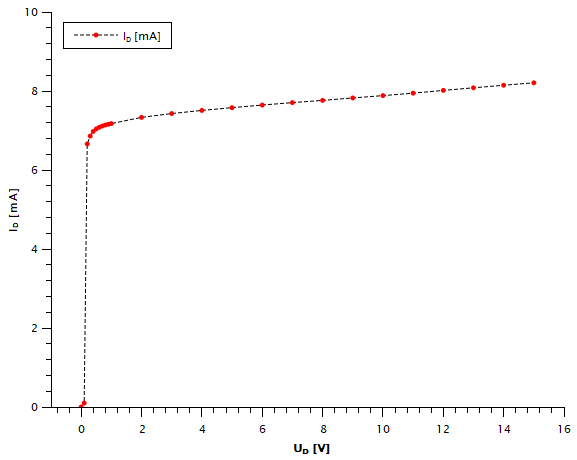
\includegraphics[width=0.8\linewidth, ]{vystup1} 
			\caption{Výstupní charakteristika při \\$U_G = 3.6V$}
			
		\end{center}		
	\end{figure} 
	Ze zadání vyučujícího jako pracovní bod uvažujeme hodnoty:
	\begin{equation}
		U_{G0} = 3.5\,\mathrm{V}, U_{D0} = 10\,\mathrm{V}, I_{D0} = 2.92\,\mathrm{mA}
	\end{equation}
	\begin{figure}[H]
		\begin{center}			
			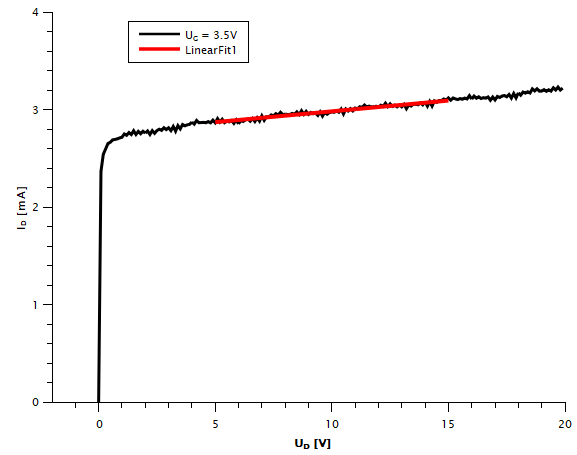
\includegraphics[width=0.8\linewidth, ]{linearfitodpor} 
			\caption{Výstupní charakteristika při \\$U_G = 3.5V$}
			
		\end{center}		
	\end{figure} 
	V obrázku 5 jsme aproximovali vnitřní odpor tranzistoru. V souladu s formulí (2) lze odpor lineárně aproximovat v okolí pracovního bodu, tedy v saturační oblasti výše křivky na obr. 5. Získáváme hodnotu odporu:
	\begin{equation*}
		R_i = 45.2\pm 1.3\,\rm k\Omega
	\end{equation*}
	
	
	Užitím formule (1) podobným postupem na závislosti $U_G$ na $I_D$ při $U_D = 10V$ získáváme hodnotu strmosti tranzistoru S:
	\begin{equation*}
		S = 29.3 \pm 0.5 \,\rm m\Omega^{-1},
	\end{equation*}
	z čehož prostřednictvím Barkhausenovy formule získáváme i zesilovací činitel $\mu$:
	\begin{equation*}
		\mu = (1.32 \pm 0.04).10^3
	\end{equation*}
	Z dat získaných počítačovým měřením vytvoříme graf výstupní charakteristiky a graficky spočítáme hodnotu zesílení $A_G$:
	\begin{figure}[H]
		\begin{center}			
			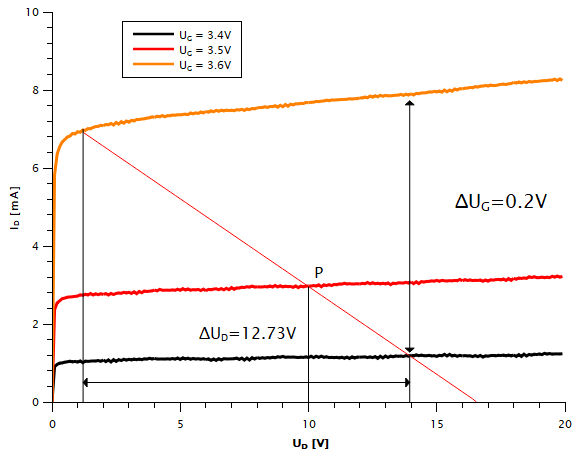
\includegraphics[width=0.8\linewidth, ]{comppomer} 
			\caption{Výstupní charakteristika s hodnotami $\Delta U_G$ a $\Delta U_D$}
			\end{center}		
	\end{figure} 
	Použitím formule (8) získáváme hodnotu zesílení\begin{center}
		$	A_G = 66.4$
\end{center}
\subsection{Tranzistor jako zesilovač napětí}
\begin{figure}[H]
	\begin{center}			
		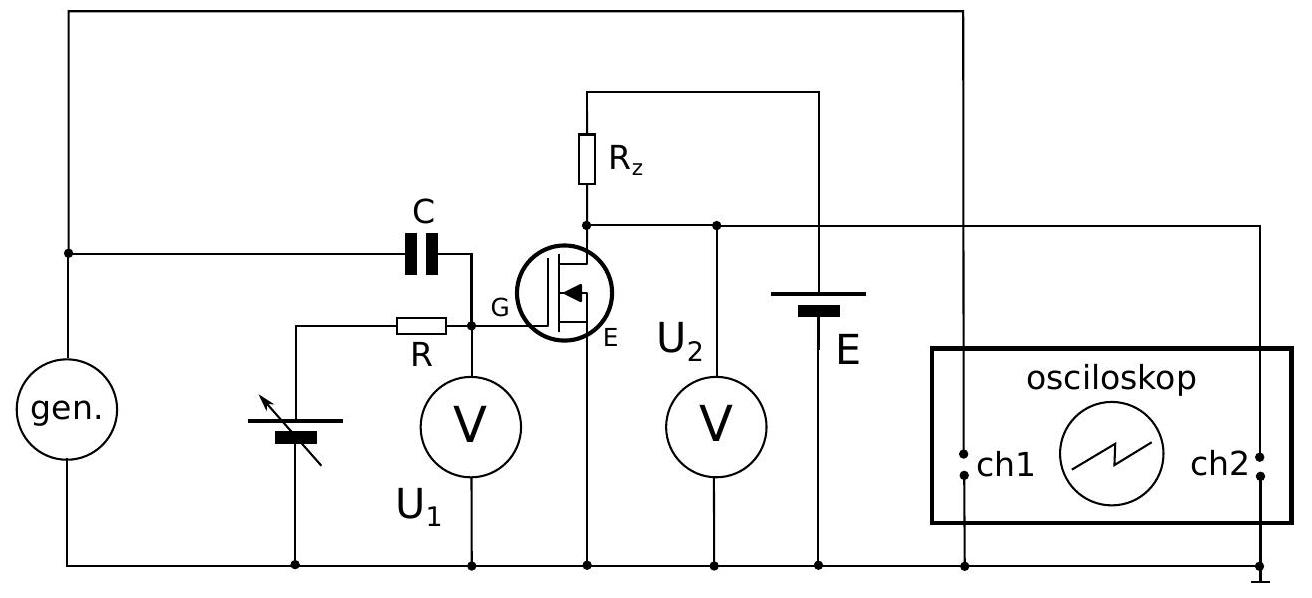
\includegraphics[width=0.8\linewidth, ]{zapojeni3} 
		\caption{Zapojení pro měření vlastností zesilovače}
	\end{center}		
\end{figure} 
Pro měření vlastností zesilovače použijeme zapojení dle Obr. 6, v souladu s formulí (6) a pracovním bodem (11) získáme hodnotu zatěžovacího odporu, přičemž uvažujeme s napětím zdroje $E$ o dvojnásobné hodnotě $U_{D0}$. Získáváme odpor $R_z$ = 3.4 \,\rm k$\Omega$. Na generátoru generujeme sinusový signál o různých frekvencích a pozorujeme, jak se mění hodnota vstupní a výstupní amplitudy:
\begin{center}
	\begin{tabular}{|c|c|c|}
	\hline
	f [kHz] & $U_{m1}$ [V] & $U_{m2}$ [mV] \\ \hline
	0.25    & 14.4         & 214           \\ \hline
	0.5     & 14.8         & 212           \\ \hline
	1       & 14.8         & 212           \\ \hline
	1.5     & 14.8         & 212           \\ \hline
	2       & 14.8         & 214           \\ \hline
\end{tabular}
\end{center}
	Pozorujeme, že jsou hodnoty amplitud nezávislé na frekvenci signálu. Hodnotu zesílení získáme použitím formule (9):
	\begin{equation*}
	A_D =	69.2 \pm 0.4
	\end{equation*}
	Hodnotu zesílení zesilovače získáme užitím formule (10):
	\begin{equation}
		A_V = 6.97 \pm 0.22
	\end{equation}
	
	\section{Závěr}
	Podařilo se nám splnit veškeré zadané úkoly a získat hodnoty hledaných veličin, přičemž vše bylo v souladu s předpokládaným chováním tranzistoru.
	
	


	

	
	% Nakonec nezapomeňte projet text programem vlna nebo vlnka, např.
	% 	vlna -m -l -n mojeuloha.tex
	% nebo zkontrolovat a opravit jednopísmenné předložky na koncích řádků ručně.
\end{multicols}
\end{document}
